\section{Scaling Architecture}

When building this system, we paid close attention to scalability. We chose AWS as a hyper-scaler platform to run our complete system. AWS provides thousands of services which are built on top of the principles of scaling and pay-what-you-use. This means if we generate intermittent load, we will only have to pay for the resources while they were in use as we do not have to provision our infrastructure for the maximum load it could ever face, and rather let it scale dynamically by demand.

Assessing the goodness of an architecture is less straightforward than evaluating forecasting accuracy. Throughout this section, we will make qualitative arguments to support our design choices by comparing it to alternative solutions and adherence to common design patterns and principles for system design and distributed computing.

\begin{figure*}
\centerline{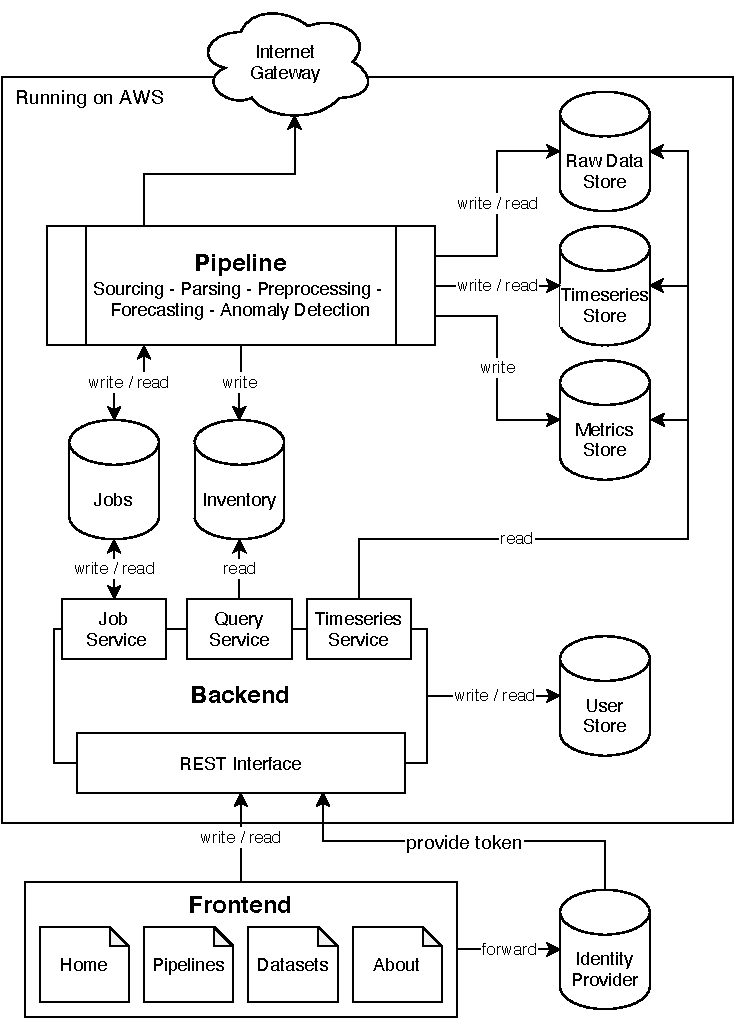
\includegraphics[scale=.7]{Figures/system-overview.pdf}}
\caption{The core components Pipeline, Backend and Frontend. All services run in an AWS datacenter.}
\label{fig:system-overview}
\end{figure*}

The diagram in figure \ref{fig:system-overview}, shows the core components pipeline, backend and frontend of the system.


\subsection{Distributed Pipelines}

Our system allows users to schedule scraping, pre-processing, forecasting and anomaly detection at any time. This means we will always have spikes in needed capacity at whatever area. Thus, we must make design choices that allow spikes to be broken down into smaller work packets that will be processed in parallel.

We propose a messaging model where events can be pushed to, and then out of it several jobs are triggered. Let's say we push ten jobs to a queue, each job then start working immediately in parallel not requiring a resource to unblock first. After a job is finished it updates the original job with its status and resource locators to the generated artifact.

Building on hyper-scaler services we can benefit from infinite amount of compute and storage resources if we implement it according to best practices. For example, a hyper-scaler such as AWS can buy more hard disks faster than a single program can write data onto such disks.

Since we want our system to have the absolute minimal costs if it's not currently in use, we also must accept some compromises. Certain open-source technologies such as Kafka cannot be provisioned on AWS without specifying a minimal broker instance type with 2 CPUs. Thus, the space of scalable messaging services is limited to services developed by AWS, if we stay with the decision to run on AWS.

Our choice for messaging and distributing the pipeline load was AWS DynamoDB\footnote{\url{https://aws.amazon.com/dynamodb/} (30-10-2021)} and AWS Lambda\footnote{\url{https://aws.amazon.com/lambda/} (30-10-2021)}. AWS DynamoDB is a proprietary document store like MongoDB. One can store documents of any shape in a table as long as they contain a partitioning key and an optional sort key. We can then enable streaming of a table to trigger events automatically by the system. In our case we trigger executions of AWS Lambda serverless functions. Lambda functions are pieces of code that do not have a known host instance. Once invoked, the platform allocates the required resources on a node and pulls the code package and executes it. After the function is done, the Lambda services keeps its allocated resources and placed code warm for a bit longer to profit from a startup boost should there be another invocation soon after. 
DynamoDB is priced with \$1.25 per million write requests, \$0.25 per million read requests and \$0.25 per GB-month. We do not need to keep logs of jobs forever and we should evict them after a while. In DynamoDB one can set a Time-To-Live (TTL) per document in a table.

In our proposed architecture, multiple actors can publish a job in a job queue of a certain type (Sourcing, Parsing, Preprocessing, Forecasting, Anomaly Detection, Model Analyzer). Each job has its own DynamoDB table, and thus we can trigger different functions based on the table. Spikes in new job creation do not matter as AWS Lambda spawns as many functions as necessary. The function invocation event also contains the content of the document itself, in this case the job description, meaning we do not need to read any job configuration upon invocation. 
The default pipeline is shown in figure \ref{fig:pipeline-diagram}.

There are three types of job creations. 

\textbf{Manual} invocation happens if the backend needs to have a job processed immediately when a user is currently configuring a pipeline and wants fast feedback. We considered storing manual jobs in a separate queue, but in the end, this is not necessary because jobs are processed immediately in any case. It would only make the architecture unnecessarily more complex. We added a preview flag to these jobs. If the flag is set, the step will only compute a partial \emph{preview} result that can be shown to the user as fast feedback to their configuration. We set the number of timeseries to be processed in a preview to a maximum of 10 first rows.

\textbf{Scheduled} invocation happens if a job has been configured to run on an interval. In our case we use the Cron \cite{cron} notation to specify a schedule. To support scheduled jobs, we need an extra piece in our architecture. We do not want to trigger the target functions directly by adding a scheduled trigger, because then they would need to get the job information in this case, and we lose our decoupling through the job queue partially. Thus, we have another function which is triggered by the configured schedules in the system. It then computes which jobs must be executed and writes them into the respective queues. Sourcing, Forecasting and Anomaly Detection steps can be triggered by a schedule. Additionally, every step that follows a pipeline join must also be triggered by a schedule.

\newpage
\textbf{Downstream} invocations happen when a step in the pipeline finishes, such as sourcing, and another step down the stream now has to process the data, e.g., the parsing step. To solve this and keep our decoupling, we added yet another function which listens to a stream of job updates of steps that can have downstream steps. We call this the scheduler function. It can then put the follow up jobs into the respective queue. There are multiple downstream steps if the pipeline is forked.

\begin{figure*}
\centerline{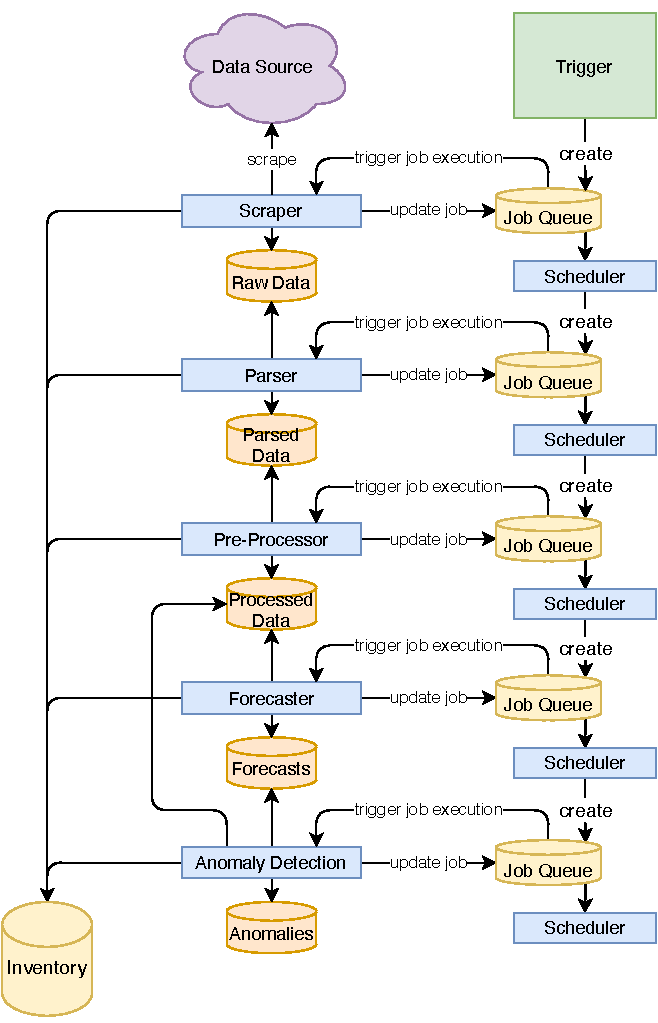
\includegraphics[scale=.7]{Figures/pipeline-diagram.pdf}}
\caption{The default pipeline is shown in this diagram. Each step can only be triggered by adding an item to the job queue. A step also never directly triggers any other steps. Everything is decoupled using message streaming. The blue boxes are implemented as AWS Lambda functions. The Orange stores are AWS S3 buckets. The yellow stores are AWS DynamoDB tables.}
\label{fig:pipeline-diagram}
\end{figure*}

We store artifacts in AWS Simple Storage Service (S3)\footnote{\url{https://aws.amazon.com/s3/} (30-10-2021)}. These artifacts are raw data scraped from a URL, processed timeseries in the form of CSV files, forecasts and anomalies also in the form of CSV files and metrics of the model's performance in the form of JSON files. The forecast CSV file contains the timeseries data used to predict it but is labeled with a flag in an extra column. The same applies for detected anomalies. The anomaly detection step will create a new CSV file with original data, forecasted data and anomalies. Each step may also update the inventory store which keeps track which dataset and which timeseries exists and where to find this data on S3. When the backend wants to display a timeseries with original data, forecast and anomalies, it only must fetch the last CSV file from S3 in a single get operation.

We are not using a timeseries database such as AWS Timestream, InfluxDB or the like. We argue that it is not necessary to have a timeseries database in our case. A timeseries database allows to make queries of timeseries data that includes filters, transformations and aggregations. We do not need to aggregate multiple timeseries, nor do we need to transform them, since our pipeline's job is to apply necessary transformations already. We need to lookup them up, but we propose to use an Inventory approach where we store the keys and labels in a DynamoDB table that can be searched. Most timeseries databases are also focused on ingestion and recent data, where they compact older data to save storage space. We do not want a database to compact old timestamps, as they might have been uploaded by a user just recently and are in high use.

\subsection{Pipeline Latency}

The data sourced is potentially many megabytes large containing thousands of timeseries. Computing a forecast on all of them at once in a single AWS Lambda function is not a good option to keep the pipeline latency low. Thus, we propose to use smaller batch sizes. Steps other than forecasting do not need batch processing as they are generally all fast or can inherently not be split. Before creating the forecasting job, we split the dataset into timeseries and group them according to their selected model which is defined in the pipeline configuration. We then create batch sizes according to the expected time per forecaster to fit and predict such that the total execution of the function remains less than 5 minutes. We have the expected durations recorded in our summaries from the model evaluation, thus we make use of them. Each function then receives a batch range that it uses to read only those timeseries from the dataset in S3. This allows us to keep the latency of the produced forecasts relatively low. Because we have now multiple functions working on the same step of the pipeline, we now have not only a pending and complete job, but each function will update the job and marking the batch as complete. The function that updates the job as the last function notices that all other batches are also complete and marks the job as fully complete. For this case it is important to use strongly consistent database reads in contrast of eventually consistent reads (which is the default for DynamoDB).

However, we run into a problem if we must create forecasts for a dataset such as the one from the Web Traffic competition with 145,000 timeseries in it. Assuming the user selects a model for all timeseries that is comparatively very slow such as 2 seconds. We then estimate a batch size of 150 to allow the function to finish within 5 minutes. This means we will spawn $145,000 / 150 = 966$ functions. The limit of AWS Lambda functions that can be running at the same time is 1,000 by default. To mitigate this, we increase the batch size for such datasets, so forecasts are ready within 15 minutes. AWS allows the increase of the concurrently running Lambda functions if necessary.

\subsection{Backend}

Our web application needs to have a backend. We propose to use the Backend-for-Frontend (BFF) design pattern. In this pattern, a frontend only ever has one backend it communicates with and vice very, the backend only has one frontend. The benefit of using this pattern is that all the endpoints can be built tailor made for the frontend and there is no need to build a generic API that does not work well for the frontend.

Our backend exposes a REST API that uses OAuth 2.0 \cite{oauth2} to protect certain endpoints which need authentication and authorization. Our technology of choice is Java and Spring Boot, however this does not really matter as other languages and frameworks are out there that do the job just as well. It is important however that these applications can be containerized and are cloud native. We are using a stateless API which means we can dynamically scale horizontally if load for the backend increases. We run our backend with AWS App Runner\footnote{\url{https://aws.amazon.com/apprunner/} (30-10-2021)}. This service handles complexities like resource pool allocation, load balancing, auto scaling and automatic deployments with a rolling strategy which does not incur any downtime when a new version is deployed. There is no need to specify or maintain a cluster. It is close to using Cloud Foundry\footnote{\url{https://www.cloudfoundry.org/} (30-10-2021)}. If we would use a popular alternative Kubernetes\footnote{\url{https://kubernetes.io/} (30-10-2021)} we would need to handle this by configuring and testing every aspect. In our scenario we do not need the flexibility that Kubernetes offers; AWS App Runner is good enough.

To expose our REST API to the frontend we configured AWS CloudFront\footnote{\url{https://aws.amazon.com/cloudfront/} (30-10-2021)} to be our entrypoint for incoming requests. The CloudFront distribution then routes requests which begin with $/api/$ to the backend URL. The backend URL points in fact to a load balancer which distributes the load between the backends and measures the traffic to do auto scaling.

\subsection{Frontend}

Above we mentioned CloudFront. If the path does not begin with $/api/$, we proxy to a S3 bucket which contains the built sources of our web application in HTML, JS and CSS files. We build these files by using Angular\footnote{\url{https://angular.io/} (30-10-2021)} as a frontend framework to implement a Single Page Application (SPA). This application allows users to sign up, configure a pipeline and inspect the resulting forecasts. The fact that this is a highly interactive website and that it communicates with a REST API lets us argue that a SPA is a good fit.

Users need to authenticate to create pipelines. We did not plan for one-off visits where a user creates one forecast and then leaves the sit and never wants to tweak their pipeline. Our system allows signing up through Google OAuth 2.0 \footnote{\url{https://developers.google.com/identity/sign-in/web/sign-in} (30-10-2021)}. The benefit is that users do not need to create an account by entering username and password. The drawback is that users need to have a Google Account. We want to extend this sign-up process to support more providers such as GitHub and provide a fallback for email and password if the user does not want to sign up using any of these identity providers.

Users can make their datasets public. This means that unauthenticated users can access these timeseries and their forecasts. This can be useful if the data is open-source and one wants to consume forecasts about certain data.
